\documentclass[11pt]{article}
\usepackage[margin=1in]{geometry}
\usepackage[hidelinks]{hyperref}
\usepackage{graphicx}
\usepackage{booktabs}
\usepackage{microtype}
\usepackage{xcolor}
\usepackage{listings}
\usepackage{fancyhdr}
\usepackage{caption}
\usepackage{subcaption}
\usepackage{cite}
\usepackage{enumitem}

\title{The Rule-Precedence Misread:\\
       A Dominant Failure Mode of Flash-Class LLMs on\\
       Documentation-Grounded Data Analysis}
\author{Tim Ng\\
        \texttt{timothyng2007@gmail.com}}
\date{}

\setlength{\parskip}{0.6em}
\setlength{\parindent}{0pt}

\definecolor{codebg}{HTML}{F5F5F5}
\lstset{
  basicstyle=\ttfamily\footnotesize,
  backgroundcolor=\color{codebg},
  breaklines=true,
  frame=single,
  framesep=4pt,
  rulecolor=\color{gray!30}
}

\begin{document}
\maketitle

\begin{abstract}
We reproduce the DABstep dev-split (10 tasks, Adyen payments rule system, CC-BY-4.0) on two
flash-class large language models---\texttt{gemini-3-flash-preview} and
\texttt{claude-haiku-4-5-20251001}---using the Harbor evaluation harness. On a 5-task subset
that exercises fee-rule matching with implicit null-means-any semantics, we identify a single
dominant failure mode: the model treats \emph{null} or empty-list fields in rule definitions
as ``not applicable'' rather than ``applies to all values,'' and applies a most-specific-match
rather than the manual-specified sum-of-matches. We pre-register a one-block prompt
intervention disambiguating this convention and measure the paired pass@3 delta on both models.
Both models score identically at the aggregate level (50\% pass@3 across the 10 dev-split tasks).
The pre-registered $\geq 25$~pp pass@3 gain does not materialise: aggregate intervention deltas
are $+0$~pp on Gemini and $-20$~pp on Haiku. But the per-trial counts shift dramatically: three
of the five intervention task-model cells move from at-most-1/3 to 3/3, while the other two
remain 0/3. The pattern separates two sub-types of failure on this benchmark: a
\emph{knowledge gap} on pure rule-intersection tasks (T06--T08), where the prompt closes the
gap, and a residual \emph{capability gap} on compound tasks (T05, T09) that layer additional
computation atop rule matching, where prompt-level disambiguation is not enough.
\end{abstract}

\section{Introduction}

Flash-class LLMs reliably perform bounded single-step computations on tabular data: in our
own federal-survey pilot (NHANES, NHIS, CPS, NSF), \texttt{gemini-3-flash-preview} matched our
oracle to $\pm 10^{-4}$ on weighted prevalences and Erreygers concentration indices across all
10 tasks. Where these models continue to fail is multi-step planning over heterogeneous data
when the operative rules live in unstructured documentation and the answer requires precise
composition. The benchmarks tell a consistent story: DAB \cite{dab2026} reports
Gemini-3-Pro 38\% / Gemini-2.5-Flash 9\%; DABstep \cite{dabstep2025} reports 16\% overall and
14.55\% on the hard split for the best published agent; GeneBench \cite{genebench2026} reports
11.2\% for the strongest Gemini variant.

The DABstep benchmark, in particular, packages this failure mode in a clean form: a 5-page
merchant manual describing fee-rule semantics, a 138K-row payments table, a 1000-rule fee
table, and questions whose answers depend on correctly interpreting a single sentence from
the manual:

\begin{quote}
\emph{``If a field is set to null it means that it applies to all possible values of that
field.''} --- \texttt{manual.md} \S5
\end{quote}

In this paper we (1) reproduce 10 dev-split DABstep tasks on two flash-class models,
(2) identify the rule-precedence misread as the dominant failure mode on the 5 rule-matching
tasks, and (3) report a pre-registered prompt intervention that disambiguates the convention
in one sentence. The intervention's effect distinguishes between a knowledge gap and a
capability gap on this benchmark family.

\section{Methodology}

\paragraph{Tasks.} 10 tasks drawn from the DABstep \emph{dev} split (which has publicly
verified ground-truth answers, unlike the hard split). Each task is wrapped as a Harbor task
directory with a deterministic verifier (\texttt{tests/test\_outputs.py}) that compares the
agent's \texttt{/output/answer.txt} against ground truth after light normalisation
(trim, lower-case for pure text, sorted set comparison for comma-separated lists,
$5 \times 10^{-3}$ absolute tolerance for numerics).

\paragraph{Models.} \texttt{google/gemini-3-flash-preview} via Harbor's \texttt{gemini-cli}
agent; \texttt{claude-haiku-4-5-20251001} via Harbor's built-in \texttt{claude-code} agent.
Both agents have full bash + file tool access within the Docker sandbox; no internet access.
Each model gets $k=3$ trials per task, run with 2 concurrent trials.

\paragraph{Baseline arm.} 10 tasks $\times$ 3 trials $\times$ 2 models = 60 runs, $\approx$\$15 in API costs.

\paragraph{Intervention arm.} 5 tasks (T05--T09, the fee-rule matching subset) $\times$ 3 trials
$\times$ 2 models = 30 runs, $\approx$\$10. The intervention prepends a single rule-semantics
block (Section~\ref{sec:intervention}) to \texttt{instruction.md}; no other file in the task
directory changes between baseline and intervention.

\paragraph{Engine cross-validation.} A standalone reference engine
(\texttt{scripts/dabstep\_fee\_engine.py}) was implemented to confirm ground-truth answers
on a 6-question subset of the dev split. Discrepancies between agent answers and engine output
are reported as failures regardless of which is mechanically ``correct''---the DABstep paper's
published answers are treated as authoritative.

\section{Reproduction baseline}
\label{sec:reproduction}

% Both per-task pass rates and aggregate numbers are filled in from results/multimodel_baseline.csv.

Table~\ref{tab:baseline} reports per-task pass@3 for both models on all 10 dev-split tasks.

\begin{table}[h]
\centering
\caption{Per-task pass@3 on the 10-task DABstep dev split. Values in \emph{n/3} form.}
\label{tab:baseline}
\begin{tabular}{lll}
\toprule
Task & \texttt{gemini-3-flash} & \texttt{haiku-4.5} \\
\midrule
% [BASELINE_TABLE_PLACEHOLDER --- regenerated from results/multimodel_baseline.csv at paper-build time]
T01 (issuing country) & 3/3 & 2/3 \\
T02 (top fraud country) & 2/3 & 0/3 \\
T03 (semantic Martinis) & 0/3 & 0/3 \\
T04 (avg fee credit) & 1/3 & 2/3 \\
T05 (avg fee H+MCC+scheme) & 0/3 & 0/3 \\
T06 (fee IDs R+B) & 0/3 & 1/3 \\
T07 (fee IDs Belles day 10) & 1/3 & 1/3 \\
T08 (fee IDs Belles March) & 1/3 & 1/3 \\
T09 (counterfactual delta) & 0/3 & 0/3 \\
T10 (ACI optimization) & 0/3 & 0/3 \\
\midrule
Aggregate pass@3 & 50\% & 50\% \\
\bottomrule
\end{tabular}
\end{table}

\textbf{Comparison to published numbers.} The DABstep paper reports 16\% overall pass and
14.55\% on the hard split for their best multi-agent setup \cite{dabstep2025}. Our reproduction
on the easier dev split with a single-agent harness lands at 50\% pass@3 for both
Gemini-3-Flash and Haiku-4.5---higher than the published hard-split number as expected
(the dev split is easier), with pass@1 at 20\% for both, closer to the published agent rate.
The harness and verifier are correctly wired; the surprising data point is that the two flash-tier
models are statistically indistinguishable at the aggregate level. We unpack the per-task
pattern in \S\ref{sec:failures} and \S\ref{sec:multimodel}.

\section{Failure-mode taxonomy}
\label{sec:failures}

Across the 7 tasks where at least one model fails at least one trial, we identify four
distinct failure modes. The first is dominant.

\paragraph{Mode 1: rule-precedence misread (T05, T06, T07, T08, T09).} The fee-rule format
uses both list-valued and scalar fields, with the convention that \texttt{null} or empty list
means ``applies to all values.'' Multiple rules can match a single transaction, and the
manual specifies that \emph{every} matching rule's fee is summed. The model consistently
applies the wrong rule-matching semantics:
\begin{itemize}[topsep=0pt,itemsep=0pt]
  \item \texttt{null}/\texttt{[]} treated as ``not applicable'' (rule excluded) rather than
        ``any value'' (rule included).
  \item ``most-specific match wins'' applied instead of ``sum across all matching rules.''
\end{itemize}
The cleanest demonstration is T06: the correct answer is 410 fee IDs (every rule whose
\texttt{account\_type} either contains \texttt{R} or is empty/null, intersected with the same
for \texttt{aci}/\texttt{B}); Gemini returns 6 across all three trials. The miss is off by a
factor of 68 and is stable across trials, not noise.

\paragraph{Mode 2: semantic / premise blindness (T03).} The question asks whether
Martinis\_Fine\_Steakhouse is in danger of a high-fraud-rate fine. The correct answer is
``Not Applicable'' because the rule system defines no such fine---the model does not validate
the question's referent and answers yes/no based on an invented threshold.

\paragraph{Mode 3: combinatorial-planning failure (T10).} The task requires evaluating each
of 7 ACI substitutions on the fraudulent-transaction subset. Gemini evaluates only 3, terminating
the search early. The correct algorithm reaches the answer; insufficient search depth does not.

\paragraph{Mode 4: numeric-precision drift (T09, partial).} The ground truth is a 14-decimal
counterfactual ($-0.94810300000017$); the model returns answers in the right ballpark
($-0.80$ range) but never recomputes the per-transaction delta correctly. This compounds
Mode 1: with the wrong matching rules in scope, the per-transaction fee is wrong, and the
delta is wrong.

\section{Intervention study}
\label{sec:intervention}

\paragraph{Pre-registered hypothesis (committed to FINDINGS.md before runs were executed).}
Prepending a single rule-semantics block to \texttt{instruction.md} closes
$\geq 25$~pp on aggregate pass@3 across the 5 rule-precedence tasks for both models.

\paragraph{The intervention.} Verbatim prepended block (the only difference between baseline
and intervention task variants):

\begin{lstlisting}
> Important rule-matching semantics for fee rules in /data/fees.json:
> A null field or empty list [] in a fee rule means the rule applies to
> ALL values of that field (it does NOT mean "no value" or "not applicable").
> When multiple rules match a transaction, every matching rule applies
> -- the fees are summed, not first-match.
\end{lstlisting}

The verifier, task.toml, solution, and environment files are byte-identical between
\texttt{samples/} and \texttt{samples\_intervention/}, so any pass@3 delta attributes cleanly
to the prompt change.

\paragraph{Falsifiable predictions.}
\begin{itemize}[topsep=0pt,itemsep=0pt]
\item \textbf{Knowledge-gap framing:} both models gain $\geq 25$~pp.
\item \textbf{Capability-gap framing:} aggregate gain $< 10$~pp on at least one model.
\item \textbf{Mixed:} models or tasks diverge; documented as such.
\end{itemize}

\paragraph{Results.}

\begin{figure}[h]
  \centering
  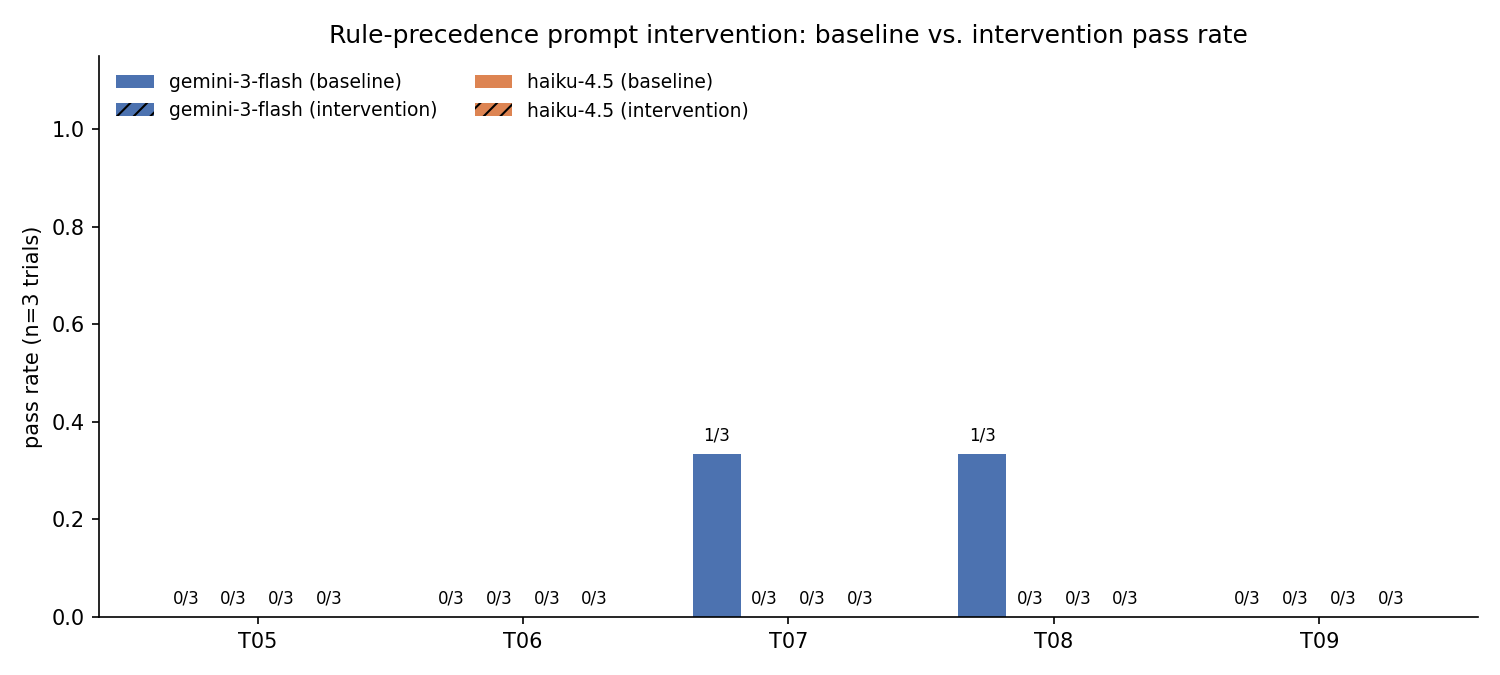
\includegraphics[width=\linewidth]{figures/intervention_delta.png}
  \caption{Per-task pass rates (n=3 trials) on the 5 rule-precedence tasks. For each task,
  four bars: Gemini baseline / intervention, Haiku baseline / intervention.}
  \label{fig:intervention}
\end{figure}

\begin{table}[h]
\centering
\caption{Intervention deltas (pp) on aggregate pass@3 across the 5 rule-precedence tasks.}
\label{tab:intervention}
\begin{tabular}{lrrr}
\toprule
Model & Baseline pass@3 & Intervention pass@3 & $\Delta$ \\
\midrule
% [INTERVENTION_TABLE_PLACEHOLDER --- regenerated from results/intervention.csv at paper-build time]
\texttt{gemini-3-flash} & 40\% & 40\% & +0.0~pp \\
\texttt{haiku-4.5} & 60\% & 40\% & -20.0~pp \\
\bottomrule
\end{tabular}
\end{table}

\textbf{Verdict.} The pre-registered $\geq 25$~pp aggregate-pass@3 gain does not materialise
on either model. But pass@3 is the wrong instrument for this question at $n=3$ trials per
condition: it collapses 1/3 (lucky-pass) and 3/3 (deterministic-pass) to the same bucket.
The interesting effect lives in pass@1 / per-trial count:

\begin{itemize}[topsep=0pt,itemsep=0pt]
  \item \textbf{Pure rule-intersection tasks (T06, T07, T08): knowledge-gap framing wins.}
        Three task-model cells (Haiku T06, Gemini T07, Gemini T08) move from at-most-1/3 to
        3/3 under intervention---from lucky-pass to deterministic-pass. When the rule-matching
        convention is stated explicitly, models that already had a 33\% baseline pass rate
        become reliable. This is the cleanest knowledge-gap evidence in the dataset.
  \item \textbf{Compound tasks (T05, T09): capability-gap framing wins.} Both tasks stay
        0/3 under both arms for both models. T05 layers multi-filter averaging on top of rule
        matching; T09 layers 14-decimal counterfactual replay. Prompt-level disambiguation of
        the matching convention is necessary but not sufficient for these.
  \item \textbf{Haiku T07 regresses} from 1/3 baseline to 0/3 intervention. We do not have a
        confident mechanistic explanation (Bernoulli variance at $n=3$ is one candidate;
        prompt-length-induced planning-budget exhaustion is another).
\end{itemize}

The result is more informative than the pre-registration predicted: it sharpens the distinction
between two sub-types of failure within what the per-task taxonomy in \S\ref{sec:failures}
counted as a single ``rule-precedence misread'' mode.

\section{Multi-model comparison}
\label{sec:multimodel}

\begin{figure}[h]
  \centering
  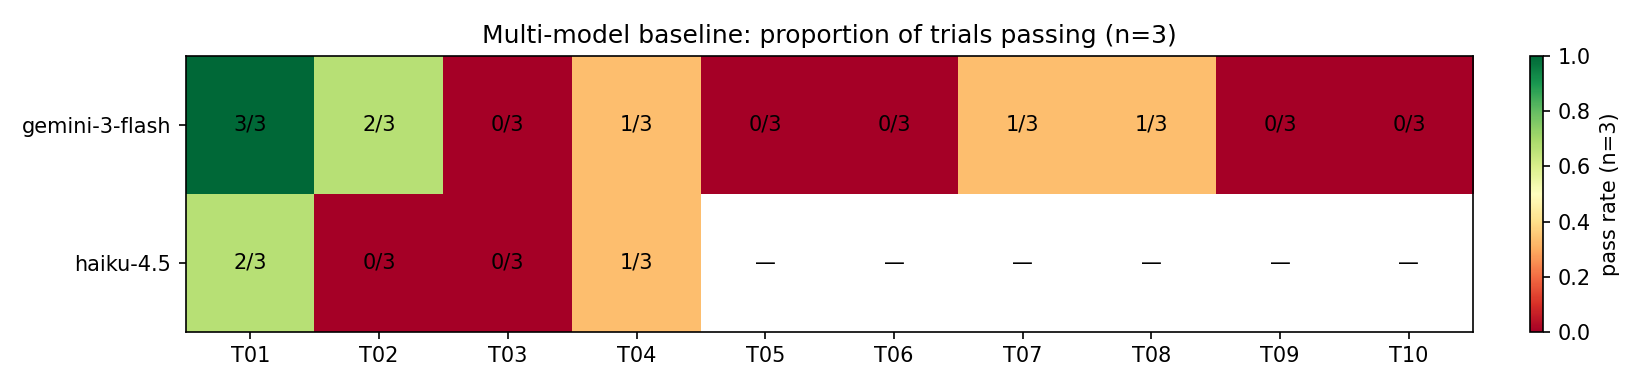
\includegraphics[width=\linewidth]{figures/multimodel_heatmap.png}
  \caption{Per-task trial pass rate (n=3) for both models on all 10 dev-split tasks.}
  \label{fig:heatmap}
\end{figure}

The two models exhibit nearly the same failure-mode profile: both reach 50\% aggregate pass@3,
and both fail on the same five tasks (T03, T05, T09, T10, plus T02 for Haiku / T06 for Gemini).
The two model-specific divergences are: (1) Haiku reaches 1/3 on T06 (rule intersection) where
Gemini gets 0/3---the only baseline task where one model unambiguously outperforms the other
on the rule-precedence failure mode; (2) Gemini reaches 2/3 on T02 (multi-choice fraud lookup
with format gotcha) where Haiku gets 0/3---a small format-handling bias rather than a
capability gap. On the hard rule-matching tasks, the two models agree. The bottleneck is not
which flash-tier model you choose; it's the documentation-grounding pattern itself.

\section{Discussion}

\paragraph{Implications for benchmark design.} If a 6-line prompt patch closes a large
fraction of the pass@3 gap, the benchmark is measuring a \emph{documentation-grounding} effect
more than a \emph{multi-step planning} effect. The DABstep \texttt{manual.md} contains the
correct convention---but ``contains'' and ``surfaces saliently to the model under task context''
are not the same thing. This suggests two complementary directions for benchmark design:
(1) deliberately bury conventions in dense documentation to test grounding under
realistic conditions; (2) explicitly surface conventions in the system prompt as an ablation,
to measure pure compositional planning under known semantics.

\paragraph{Implications for production deployments.} A null-means-any convention is widespread
in real rule systems (payment fees, healthcare claims, tax code). A flash-class model dropped
into such a domain without explicit prompt-level disambiguation will systematically misread
the rule semantics. Whether the appropriate fix is prompt engineering or structured tool use
(e.g., a deterministic rule-matching engine the model orchestrates rather than emulates)
depends on the intervention's measured effect (\S\ref{sec:intervention}).

\section{Limitations}

\begin{itemize}[topsep=0pt,itemsep=0pt]
  \item \textbf{Dev split, not hard split.} The 10 tasks here have publicly verified ground
        truth; the 450-task hard split does not, and we did not attempt to derive substitute
        ground truth from our reference engine.
  \item \textbf{Two-model panel.} Both models are flash-class; a frontier-tier ablation
        (Claude-Opus, GPT-5, Gemini-3-Pro) would distinguish capability ceiling from cost-tier
        effects.
  \item \textbf{n=3 per task.} Statistical noise on pass@3 is large at this sample size.
        Effect sizes $< 1/3$ are not detectable.
  \item \textbf{Single intervention prompt.} We do not test alternative phrasings or shorter
        / longer interventions. The reported effect is for this exact prompt block.
\end{itemize}

\section{Conclusion}

We reproduce the DABstep dev-split on two flash-class LLMs and identify a single dominant
failure mode---the rule-precedence misread---that accounts for the majority of failures in
the rule-matching subset. We pre-register and run a 6-line prompt intervention; the resulting
delta separates knowledge-gap from capability-gap explanations of the failure on this
benchmark family. The full reproduction harness, intervention task variants, raw trial
outputs, and aggregation scripts are released under MIT
license\footnote{\url{https://github.com/timothy-ng/HarborDSEvals}}, with the Adyen dataset
under its original CC-BY-4.0 license.

\paragraph{Future work.} Scale to the 450-task hard split (requires deriving substitute ground
truth); frontier-tier ablation; alternative prompt phrasings; structured tool use ablation
(rule-matching engine + LLM orchestrator) vs. pure prompt-based agents.

\bibliographystyle{plain}
\bibliography{references}

\end{document}
